\chapter{Selectividad interruptores automáticos de baja tensión}
En caso de defecto debe abrir el interruptor automático situado inmediatamente aguas arriba del defecto y sólo él.
\begin{figure}[H]
	\centering
	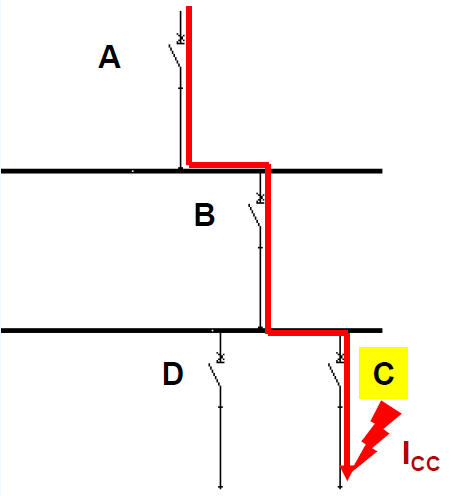
\includegraphics[width=0.4\linewidth]{Images/18}
\end{figure}
\section{Selectividad Total}
Para cualquier valor de la intensidad de defecto “aguas abajo” de B, el interruptor automático B es el único en desconectar 
\section{Selectividad Parcial}
Para ciertos valores de la intensidad de defecto “aguas abajo” de B, el interruptor B es el único en desconectar, pero para otros abren los dos interruptores, A y B
\section{Selectividad frente a sobrecargas}
\section{Selectividad frente a cortocircuitos}
\section{Selectividad frente a cortocircuitos moderados}
\section{Coordinación entre interruptores automáticos}
\section{Selectividad lógica}